%! Author = arqfa
%! Date = 2/7/2024

\documentclass[final,5p,times]{elsarticle}

%!Packages
%% The amssymb package provides various useful mathematical symbols
\usepackage{amssymb}
%% The amsthm package provides extended theorem environments
\usepackage{amsthm}
\usepackage{graphicx}
\usepackage{tabularx}
\usepackage{booktabs}
\usepackage{amsmath} % for equations
\usepackage{breakurl}
\usepackage{hyperref} % Ensure hyperlinks work properly


%% The lineno packages adds line numbers. Start line numbering with
%%\begin{linenumbers}, end it with \end{linenumbers}. Or switch it on
%% for the whole article with \linenumbers
\usepackage{lineno}
\modulolinenumbers[10]
\usepackage{enumitem}

%\usepackage{amsmath}

\usepackage{multirow}

\usepackage{caption}


% Document
\begin{document}

\begin{table*}[htb]
    \centering
    \small
    \begin{tabular}{c}
        %Top cell with one figure
        %Figure early timeline
        \begin{minipage}{\textwidth}
            \centering
            \includegraphics[width= \linewidth]{Images/OldTimeline}
                    \captionof{figure}{Early timeline. Sequential representation of architectural styles illustrating the shift between complexity and simplicity. From left to right: Romanesque[a] with its solid and massive structure; Gothic[b] featuring verticality and lightness; Classicism[c] characterized by geometrical clarity and order; Baroque[d] with dynamic shapes and rich decorations; followed by the restrained and symmetrical formality of Neo-classicism[e]. (\textit{Images edited from source})}
                    \label{fig:Oldtimeline}
        \end{minipage}
        \\
        %Middle cell
        %Middle timeline
        \begin{minipage}{\textwidth}
            \centering
            \includegraphics[width= \linewidth]{Images/MiddleTimeline}
                    \captionof{figure}{Transitional timeline. Sequential representation of architectural styles illustrating the shift between complexity and simplicity. From left to right: Art Nouveau[a] with its fluid lines and natural forms; Art Deco[b], marked by bold geometry and opulence; Modernism's[c] pursuit of stripped-back functionality; culminating in Postmodernism's[d] revival of historical styles and complexity (\textit{Images edited from source})}
                    \label{fig:Middletimeline}
        \end{minipage}
        \\
        %bottom Cell
        %Contemporary timeline
        \begin{minipage}{\textwidth}
            \centering
            \includegraphics[width= \linewidth]{Images/contemporaryTimeline}
                    \captionof{figure}{Contemporary timeline. Sequential representation of architectural styles illustrating the shift between complexity and simplicity. Era of exploration and innovation. From left to right: Deconstructivism[a], characterized by fragmentation and non-linear design; Neofuturism[b], capturing movement and technology-infused aesthetics; High-tech modernism[c], focusing on visible structural elements and technological expression; Parametricism[d], with its algorithm-based complex forms; and Pragmatic utopianism[e], blending idealistic designs with practical applications (\textit{Images edited from source})}
                    \label{fig:contemporarytimeline}
        \end{minipage}
    \end{tabular}
\end{table*}


%! Function for complexity score
%%Table function 1 complexity score
\begin{table*}[htb]
\centering
\caption{Function 1: Complexity scoring function that integrates various criteria to assess intricacy of a building facade.}
\label{tab:ComplexityScoreFunction_table}
    \begin{tabular}{|c c|}%{|c|c|}
    \hline
    % First Cell (Top-Left)
    % f1: Valid Position finder function
        \begin{minipage}{.45\linewidth}
            \centering
            \small
            \begin{tabular}{p{8cm}}
                \\
                \textbf{\(f_1\), Unified `Complexity Scoring' function 1}\\
                    \textit{Calculate the complexity score for all the images on the data pool}
                    \\
                    \begin{equation}
                        f_1(x) = \left[ \mathrm{round}\left(\sum_{i=1}^{n} w_i \cdot a_i, 2\right) \right] = complexity\_score
                    \label{eq:F1_ComplexityScoreFunction}
                    \end{equation}
                    \\
                    \textit{ for the Buildings included in the database.}\\
                \\
            \end{tabular}
        \end{minipage}
        &
        % Second Cell (Top-Right)
        % continuation f1
        \begin{minipage}{.45\linewidth}
            \centering
            \small
            \begin{tabular}{p{8cm}}
                \\\\
                \textit{where;} \\
                \(n \); is the number of performance indicators \\
                \(w_i \); represents the i-th elements weight input and \\
                \(a_i \); represents the i-th normalized score for the respective metric(`Edge Density' and `Contour Count').\\
                \\
                \textit{Finally, the `Complexity score' is assigned to each building for data visualization.}\\
                \\
            \end{tabular}
        \end{minipage}
    \hline
    \end{tabular}
\end{table*}


%!%!%Figures of 3D modeling and VR integration
%Figures "3d model vs real" and "Interior vs Exterior"
        \begin{table*}[htb]
            \centering
            \small
            \begin{tabular}{c}
                %Top cell with two figures
                \begin{minipage}{\textwidth}
                    \centering
                    % Left figure
                    %% Figure Real vs 3d Model
                    \begin{minipage}{0.49\textwidth}
                        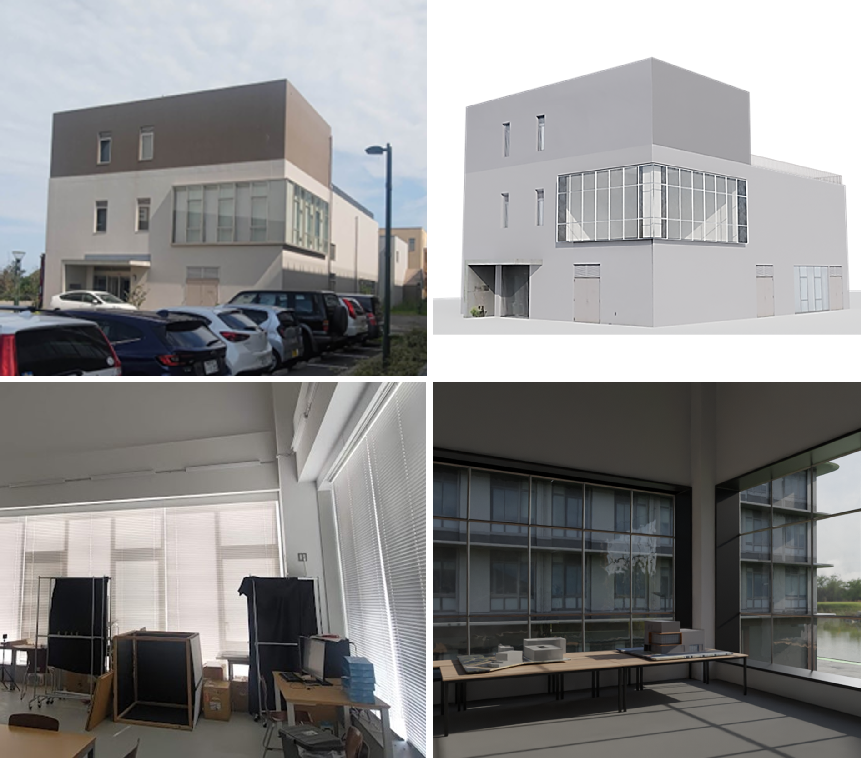
\includegraphics[width= \linewidth]{Images/Realvs3DmodelBlender}
                        \captionof{figure}{Real vs. 3D modeled building for the Facade Design Complexity Analysis experiment.}
                        \label{fig:RealVs3dModel}
                    \end{minipage}
                    \hfill % Spacing between the figures
                    % Right figure
                    %% FigureVR interior vs Exterior
                    \begin{minipage}{0.49\textwidth}
                        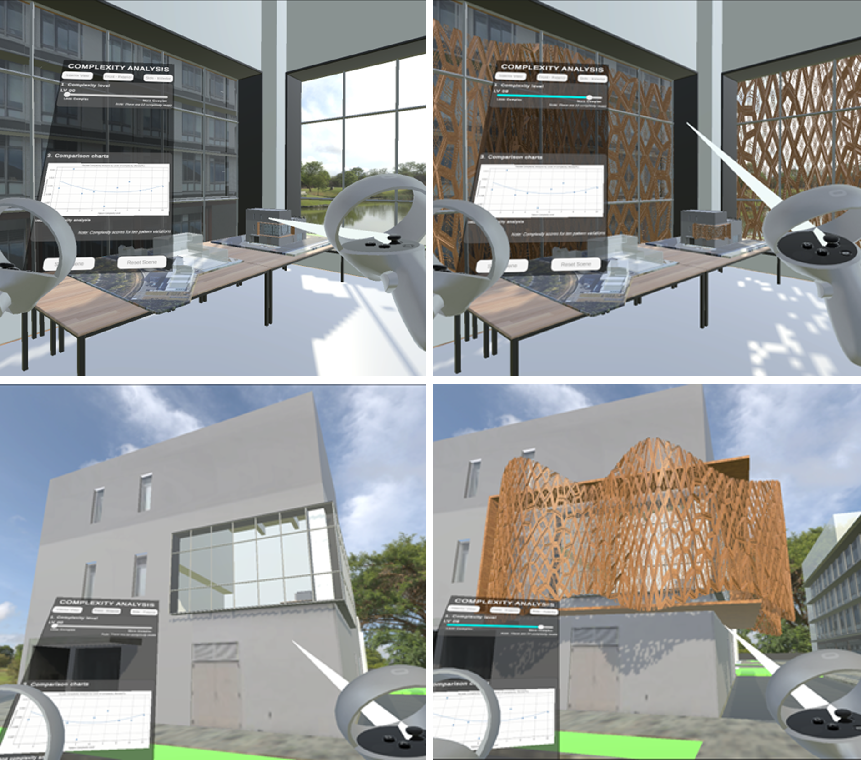
\includegraphics[width= \linewidth]{Images/VRInteriorExterior}
                        \captionof{figure}{Comparison side by side of the VR simulation of interior and exterior of existing laboratory building used for experiment (Left) and VR Simulation of facade variation (Right) used for complexity Analysis.}
                        \label{fig:VRInteriorExterior}
                    \end{minipage}
                \end{minipage}
            \end{tabular}
        \end{table*}


%!%Figures and table CICA
        %Flowchart CICA, Figure of Cica on historical buildings and renders, PI table. Table 1x3
        \begin{table*}[htb]
            \centering
            \small
            \begin{tabular}{c}
                %Top cell with one figure
                %Figure Computational Image Compexity Analysis (CICA) System flowchart
                \begin{minipage}{\textwidth}
                    \centering
                    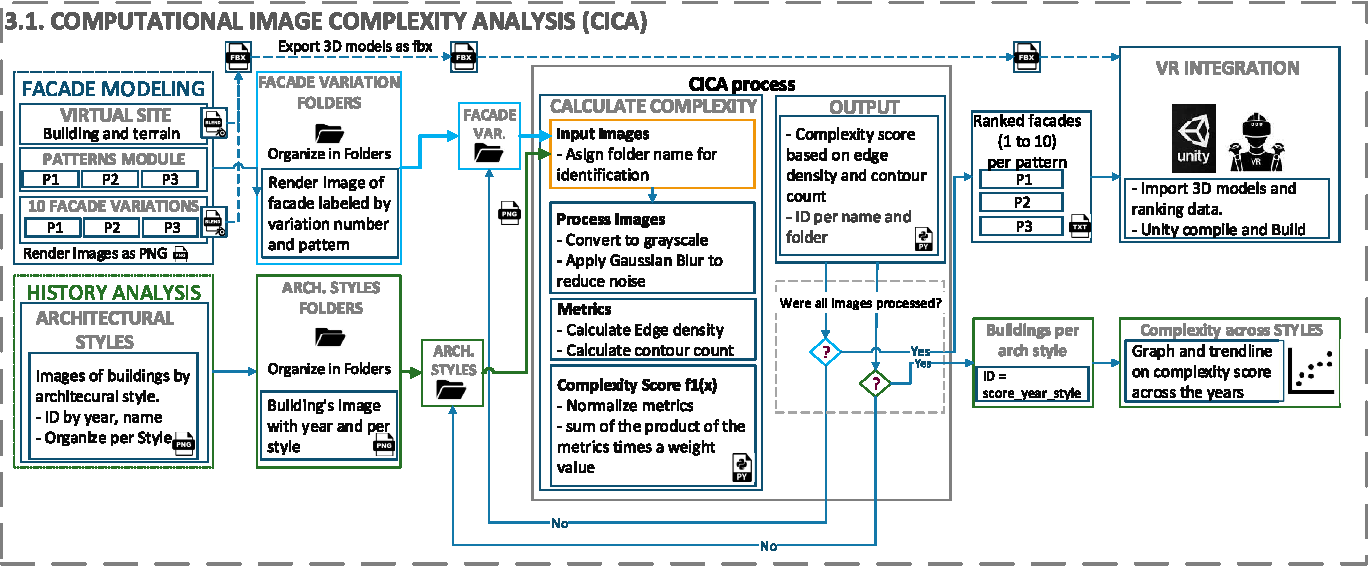
\includegraphics[width= \linewidth]{Images/ImageComplexityAnalysisFlowchart}
                    \captionof{figure}{Flowchart illustrating the applications of Computational Image Complexity Analysis, including its role in analyzing complexity scores for historical architectural styles and ranking modeled facades for the VR Building Complexity System.}
                  \label{fig:ImageComplexityAnalysisFlowchart}
                \end{minipage}
                \\
                %Middle cell with two nested figures side by side
                %%%Figure CICA on historic buildings and renders. Table 1x2
                \begin{minipage}{\textwidth}
                    \centering
                    % Left figure
                    \begin{minipage}{0.49\textwidth}
                        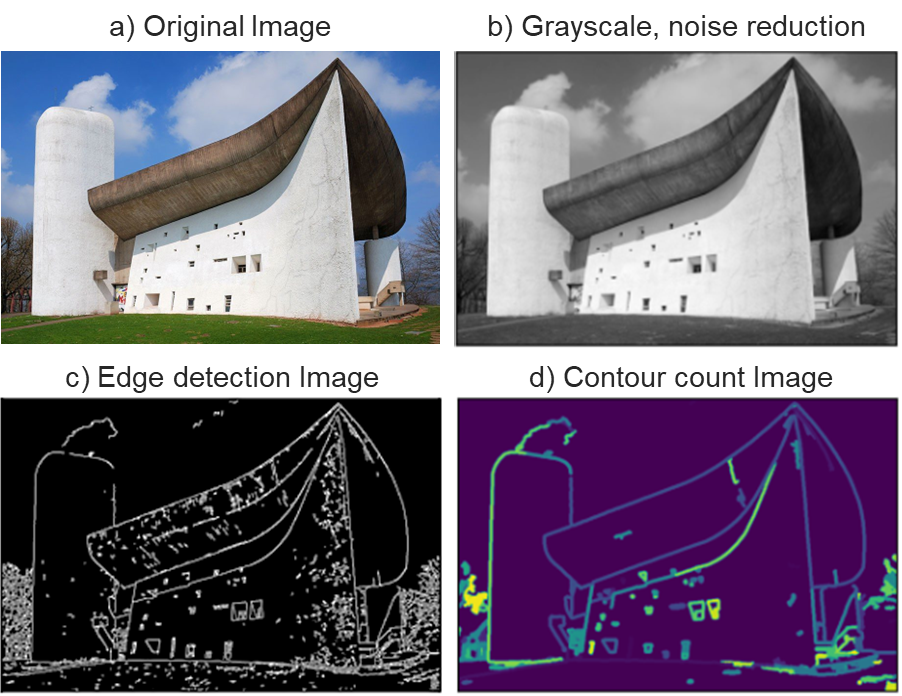
\includegraphics[width= \linewidth]{Images/CICAHistoryPlot}
                        \captionof{figure}{Edge Detection analysis of historic buildings demonstrating complexity assessment.}
                        \label{fig:ComplexityPlotHistory}
                    \end{minipage}
                    \hfill % Spacing between the figures
                    % Right figure
                    \begin{minipage}{0.49\textwidth}
                        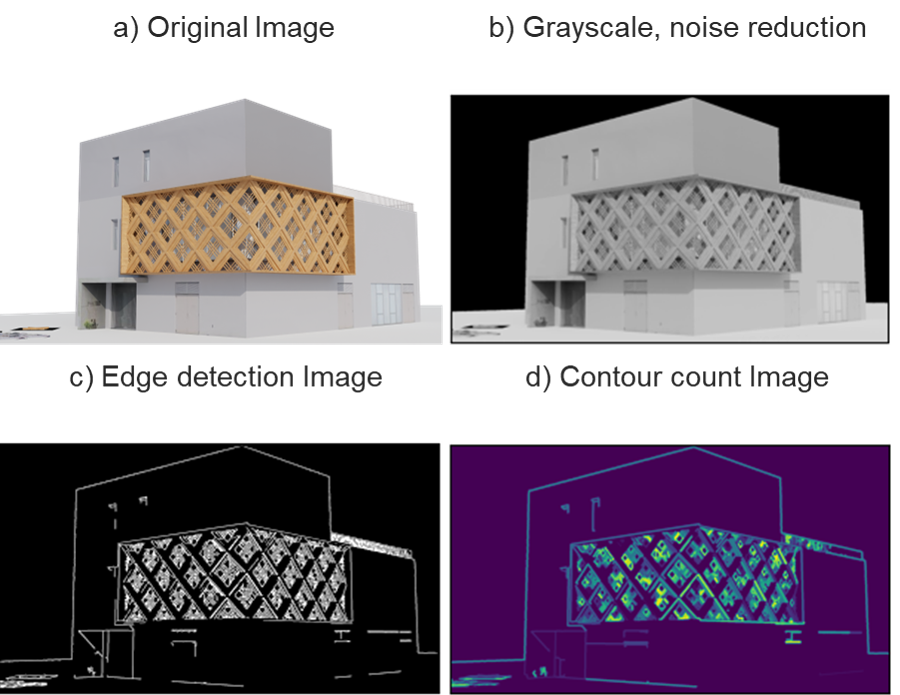
\includegraphics[width= \linewidth]{Images/CICARenderPlot}
                        \captionof{figure}{Complexity analysis of 3D-modeled facades for the VR experiment.}
                        \label{fig:ComplexityPlotRenderCICA}
                    \end{minipage}
                \end{minipage}
                \\
                %Bottom cell
                %Table: Performance Indicators
                \begin{minipage}{\textwidth}
                    \centering
                    \captionof{table}{Metrics and weights for the calculation of the `Complexity score'}
                    \label{tab:MetricsandWeights}
                    \begin{tabularx}{\textwidth}{p{3.5cm} p{1cm} X X p{1cm}}
                        \toprule
                        \textit{Complexity metric} &
                          \textit{N} &
                          \textit{Metric name/description} &
                          \textit{Quantitative   method} &
                          \textit{Weights} \\ \midrule
                        \textbf{Edge Density} &
                          1 &
                          Edge detection using Canny Edge Detection algorithm for highlighting the most relevant features of a building.
                            &
                          Measured by dividing the number of non-zero (edge) pixels in the edges image by the total number of pixels in the image.
                            &
                          8\\
                        \textbf{Contour count} &
                          2 &
                          Employs contour approximation algorithm for shape analysis to determine intricacy of edges.
                            &
                          Measure by counting the number of segments in an edge.
                            &
                          2\\ \bottomrule
                           &
                           &
                          \textbf{TOTAL} &
                          &
                          \textbf{10}\\ \bottomrule
                    \end{tabularx}
                \end{minipage}
                \\
                %Bottom cell with one figure
                \begin{minipage}{\textwidth}
                    \centering
                    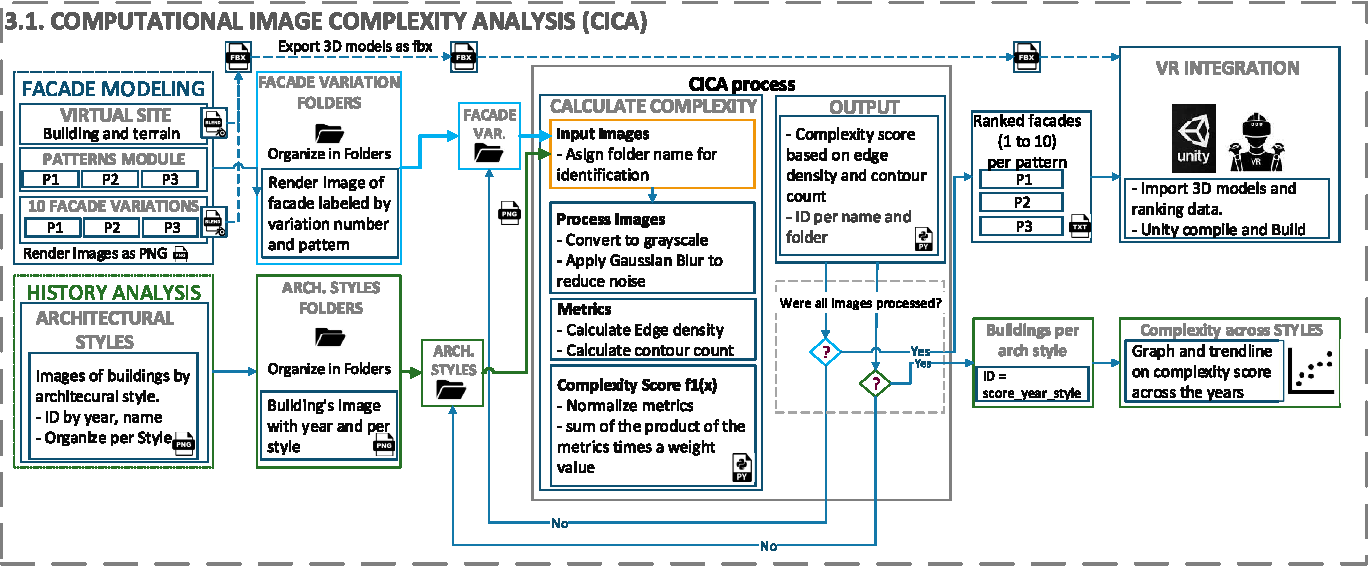
\includegraphics[width= \linewidth]{Images/ImageComplexityAnalysisFlowchart}
                    \caption{Flowchart illustrating the applications of Computational Image Complexity Analysis, including its role in analyzing complexity scores for historical architectural styles and ranking modeled facades for the VR Building Complexity System.}
                  \label{fig:ImageComplexityAnalysisFlowchart}
                \end{minipage}
            \end{tabular}
        \end{table*}


%!BackUp CICA
        %% Figure Computational Image Compexity Analysis (CICA) System flowchart
            \begin{figure*}[!htb]
                \centering
                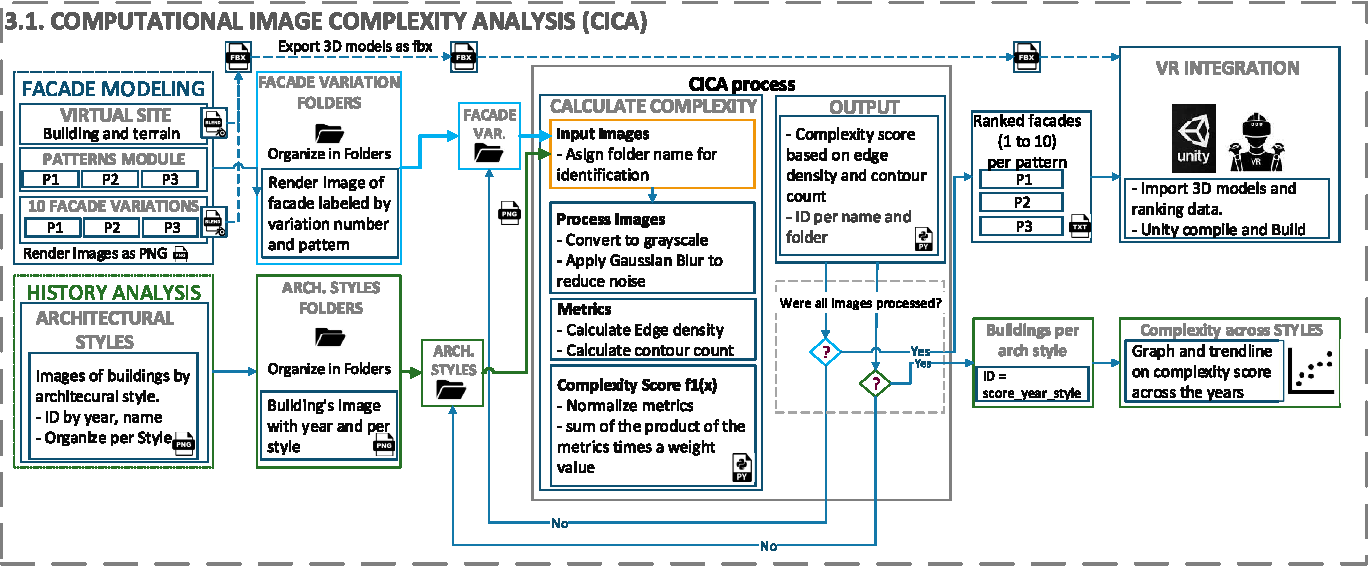
\includegraphics[width= \linewidth]{Images/ImageComplexityAnalysisFlowchart}~\caption{Flowchart illustrating the applications of Computational Image Complexity Analysis, including its role in analyzing complexity scores for historical architectural styles and ranking modeled facades for the VR Building Complexity System.}
                  \label{fig:ImageComplexityAnalysisFlowchart}
            \end{figure*}

            %%Figure CICA on historic buildings and renders. Table 1x2
            \begin{table*}[htb]
                \centering
                \small
                \begin{tabularx}{\textwidth}{X X}
                    \centering
                    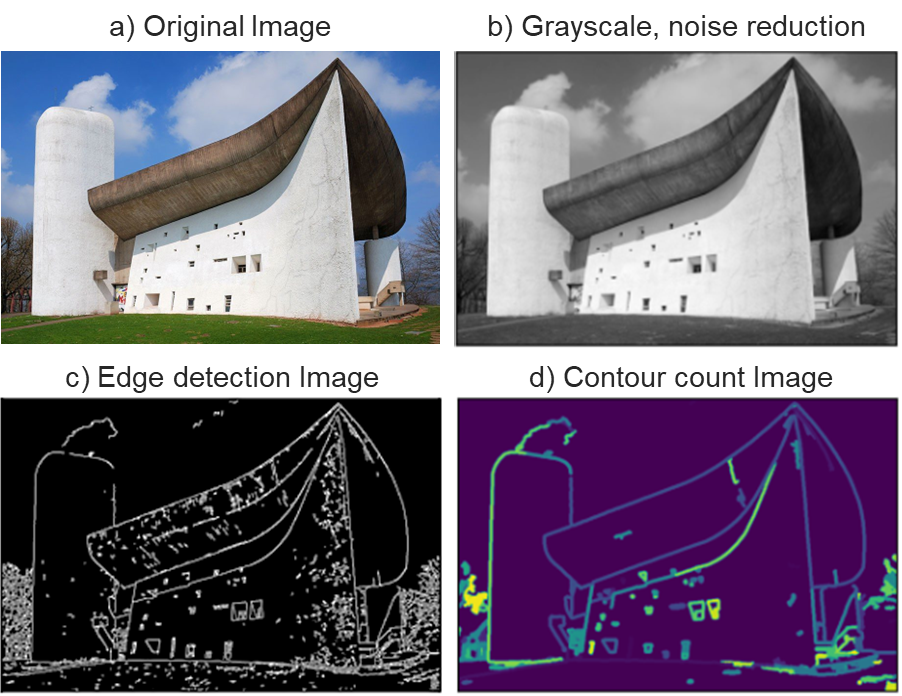
\includegraphics[width= \linewidth]{Images/CICAHistoryPlot}
                    \captionof{figure}{Edge Detection analysis of historic buildings demonstrating complexity assessment.}
                    \label{fig:ComplexityPlotHistory} &
                    \centering
                    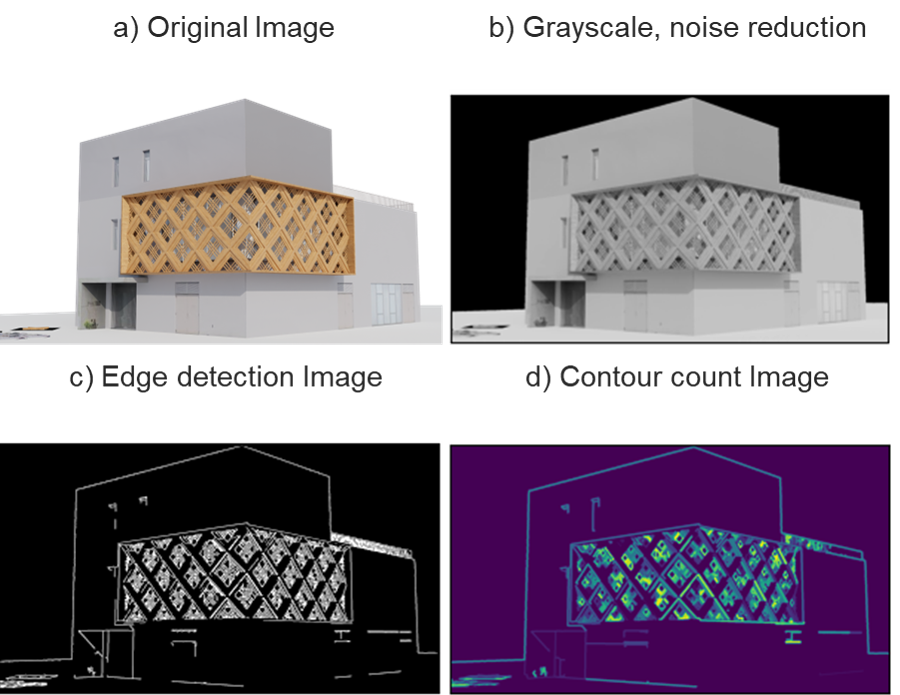
\includegraphics[width= \linewidth]{Images/CICARenderPlot}
                    \captionof{figure}{Complexity analysis of 3D-modeled facades for the VR experiment.}
                    \label{fig:ComplexityPlotRenderCICA}
                    \end{tabularx}
                \end{table*}

            %%Table: Performance Indicators
            \begin{table*}[htb]
                \centering
                \small
                \caption{Metrics and weights for the calculation of the `Complexity score'}
                \label{tab:MetricsandWeights}
                \begin{tabularx}{\textwidth}{p{3.5cm} p{1cm} X X p{1cm}}
                    \toprule
                    \textit{Complexity metric} &
                      \textit{N} &
                      \textit{Metric name/description} &
                      \textit{Quantitative   method} &
                      \textit{Weights} \\ \midrule
                    \textbf{Edge Density} &
                      1 &
                      Edge detection using Canny Edge Detection algorithm for highlighting the most relevant features of a building.
                        &
                      Measured by dividing the number of non-zero (edge) pixels in the edges image by the total number of pixels in the image.
                        &
                      8\\
                    \textbf{Contour count} &
                      2 &
                      Employs contour approximation algorithm for shape analysis to determine intricacy of edges.
                        &
                      Measure by counting the number of segments in an edge.
                        &
                      2\\ \bottomrule
                       &
                       &
                      \textbf{TOTAL} &
                      &
                      \textbf{10}\\ \bottomrule
                \end{tabularx}
            \end{table*}

%%%%%%%%%%%%%%%%%%%%
\end{document}